\newpage
\section{Documentation for programmers}
\subsection{Specification}
The program implements a DHCP relay. Figure~\ref{fig:dhcp} depicts how it works.
\begin{figure}[h]
	\centering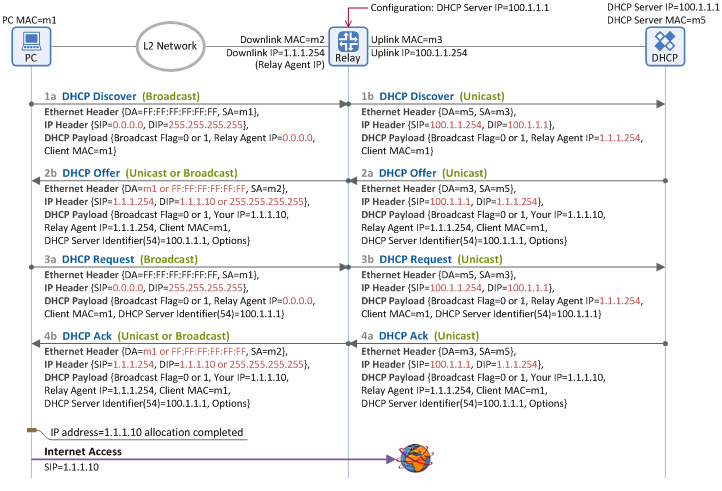
\includegraphics[scale=0.58]{images/dhcp}
	\caption{Example of DHCP protocol communication\protect\footnotemark}
	\label{fig:dhcp}
\end{figure}
\footnotetext{\url{https://www.netmanias.com/en/?m=view\&id=techdocs\&no=6000}}

Basically, a DHCP relay is a ``man in the middle'' between the client and the DHCP server. It helps the client to contact the server in order to obtain an IP address. It does so receiving the broadcast packets sent by clients and forwarding them in an unicast connection to one (or more) DHCP servers, and vice versa, forwarding the server responses in broadcast to the clients. 

While modeling its behavior, we refer to the above figure. We suppose to be able to detect when a message comes from a client and when it comes from a server by means of two different interruptions, without looking at the \texttt{OPCode} field (which is 1 for a request and 2 for a response). In other words, two \textit{different events} occur. This is reasonable, since Figure~\ref{fig:dhcp} depicts two different links (\textit{Downlink} and \textit{Uplink}), with two different MAC and IP addresses.\\

Our ASG diagram is depicted in Figure~\ref{fig:asg}.

\begin{figure}[h]
	\centering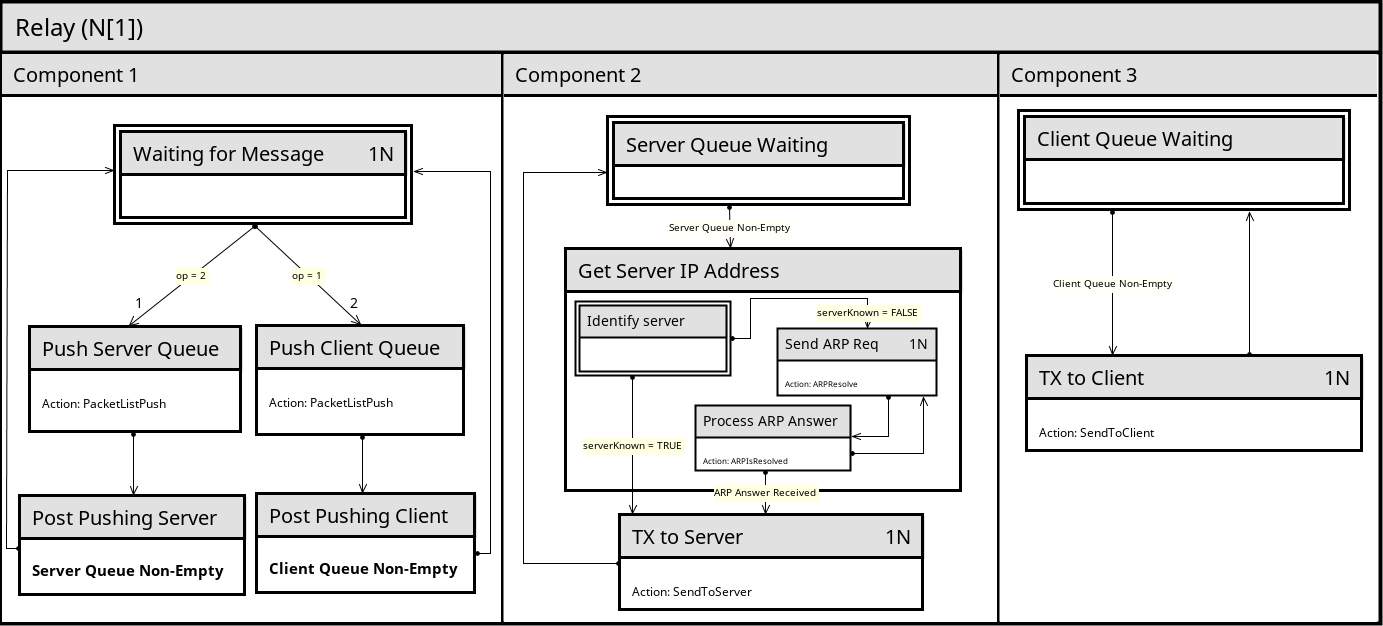
\includegraphics[scale=0.5]{images/asg-diagram}
	\caption{ASG diagram modeling a DHCP relay}
	\label{fig:asg}
\end{figure}

The DHCP relay consists of four parallel components following a producer-consumer pattern. Two components, 1 and 3, wait for a packet, either from a client (broadcast) or a server (unicast). They then modify this packet as follows:
\begin{itemize}
	\item \textbf{Component 1} - \texttt{ModifyServerPacket}:
	\begin{itemize}
		\item \textbf{Ethernet Payload}
		\begin{itemize}
			\item Destination MAC Address: DHCP Relay Uplink MAC $\to$ Broadcast
			\item Source MAC Address: DHCP Server MAC $\to$ DHCP Relay MAC Address
		\end{itemize} 
			\item \textbf{IP Payload}
		\begin{itemize}
			\item Source IP Address: DHCP Server IP Address $\to$ DHCP Relay Downlink IP
			\item Destination IP Address: DHCP Relay Downlink IP $\to$ Broadcast
		\end{itemize}	
	\end{itemize}
	\item \textbf{Component 2} - \texttt{ModifyClientPacket}:
	\begin{itemize}
		\item \textbf{Ethernet Payload}
		\begin{itemize}
			\item Destination MAC Address: Broadcast $\to$ DHCP Server MAC
			\item Source MAC Address: PC MAC Address $\to$ DHCP Relay Uplink MAC 
		\end{itemize}
		\item \textbf{IP Payload}
		\begin{itemize}
			\item Source IP Address: 0.0.0.0 (no IP address) $\to$ DHCP Relay Uplink IP
			\item Destination IP Address: Broadcast $\to$ DHCP Server IP
		\end{itemize}
		\item \textbf{DHCP Payload}
		\begin{itemize}
			\item Gateway IP Address (GIADDR): 0.0.0.0 $\to$ DHCP Relay Downlink IP
		\end{itemize}
	\end{itemize}
\end{itemize}

The two components then push the modified packet in a queue (two different queues are present, respectively for server and client) and set a rendez-vous (respectively \textbf{Client New Message} and \textbf{Server New Message}) to awake the corresponding consumer.

Component 2 and 4 represent the consumers. If they are waiting, they are awoke by a push of the corresponding producer. Once a message is received, they enter the transmission state, and leave it only when the queue is empty. Here they continuously pop an element from the queue and send it in broadcast (Component 2) or in unicast to one (or more) DHCP servers (Component 4).

This separation in two producers-consumers allow us to separate two logical different operations: handling the traffic incoming client-side and the one incoming server-side.

\newpage
\subsection{LCD non-blocking module}
The key concept in multitasking real-time systems is that tasks must be "small enough", in order not to prevent the processor for executing other operations.
In this project it is required to use the LCD display to print information messages, but the C functions provided by Microchip are not optimized for multitasking and take a non negligible time to be processed; the \texttt{LCDBlocking} module has been thus converted in \texttt{LCDNonBlocking} and integrated into the TCP/IP stack to provide a better display handling in an environment with different tasks.\\

The most time-demanding functions in the LCD library (\texttt{LCDInit}, \texttt{LCDErase}, \texttt{LCDUpdate}) have been \textbf{split in smaller states}. When called, the LCD task can only execute a part of a function: the following ones are executed at successive task calls; furthermore, each state can be accessed only if a sufficient amount of time has passed from the previous one, in line with what happened in the original file where some delays were placed between instructions.\\

\begin{wrapfigure}{l}{3.5cm}
	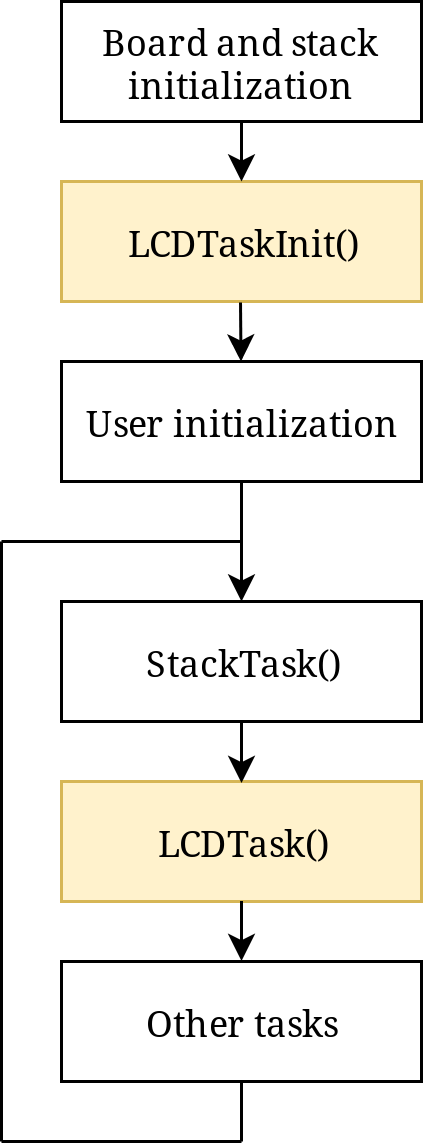
\includegraphics[width=3cm]{images/taskmgmt}
	\label{fig:taskmgmt}
\end{wrapfigure}

The main functions of the new library are \texttt{LCDTaskInit} and \texttt{LCDTask}. The first one is an initialization function which is used to assign default values to control variables and configure the resources needed for the correct operation handling. The latter is the proper task, which runs inside the cooperative multitasking loop.\\
These functions are called in the main entity as a design choice, but they could have also been integrated into the \texttt{StackTsk} file of the TCP/IP stack.\\

The big difference between the new library and the old one is that the operations are not executed immediately but are ``appended'' somewhere, so that the task can pick and perform them in successive steps without losing information about other operation requests happening in the meanwhile.\\
In order to do this, a \textbf{circular list} (actually, a circular array of structures) has been implemented: each time an \textit{Init}, \textit{Erase} or \textit{Update} operation is required, the list is filled with a code representing that operation and the text to write, if needed; this guarantees that the display always reflects the correct history of operations regardless of the state of the shadow copy.\\
The circular list static allocation required the availability of more than 256 bytes in memory, that is the maximum dimension allowed by default due to internal division of databanks in the PIC18. To overcome this limitation, the linker script was modified to create a single databank of twice the size and a \texttt{\#pragma} directive was introduced to memorize the list in that exact memory location; the solution was fully tested and does not introduce any kind of issue.\\


The delay handling is entrusted to \textbf{Timer 1} (external 32.768 kHz oscillator) because it is not used by any other part of the system; the timer is in a bounded configuration and the initial value of the register is calculated according to the necessary minimum delay for each stage. If such a waiting condition is active, the LDC task checks for an overflow of the timer register before proceeding to the execution.\\

The instruction flow of the LCD task is represented in the next page; it is a simple diagram which is not meant to explain the detailed content of each block but the general behavior of the module. For in-depth analysis it is possible to read the code.

\begin{figure}
	\centering
	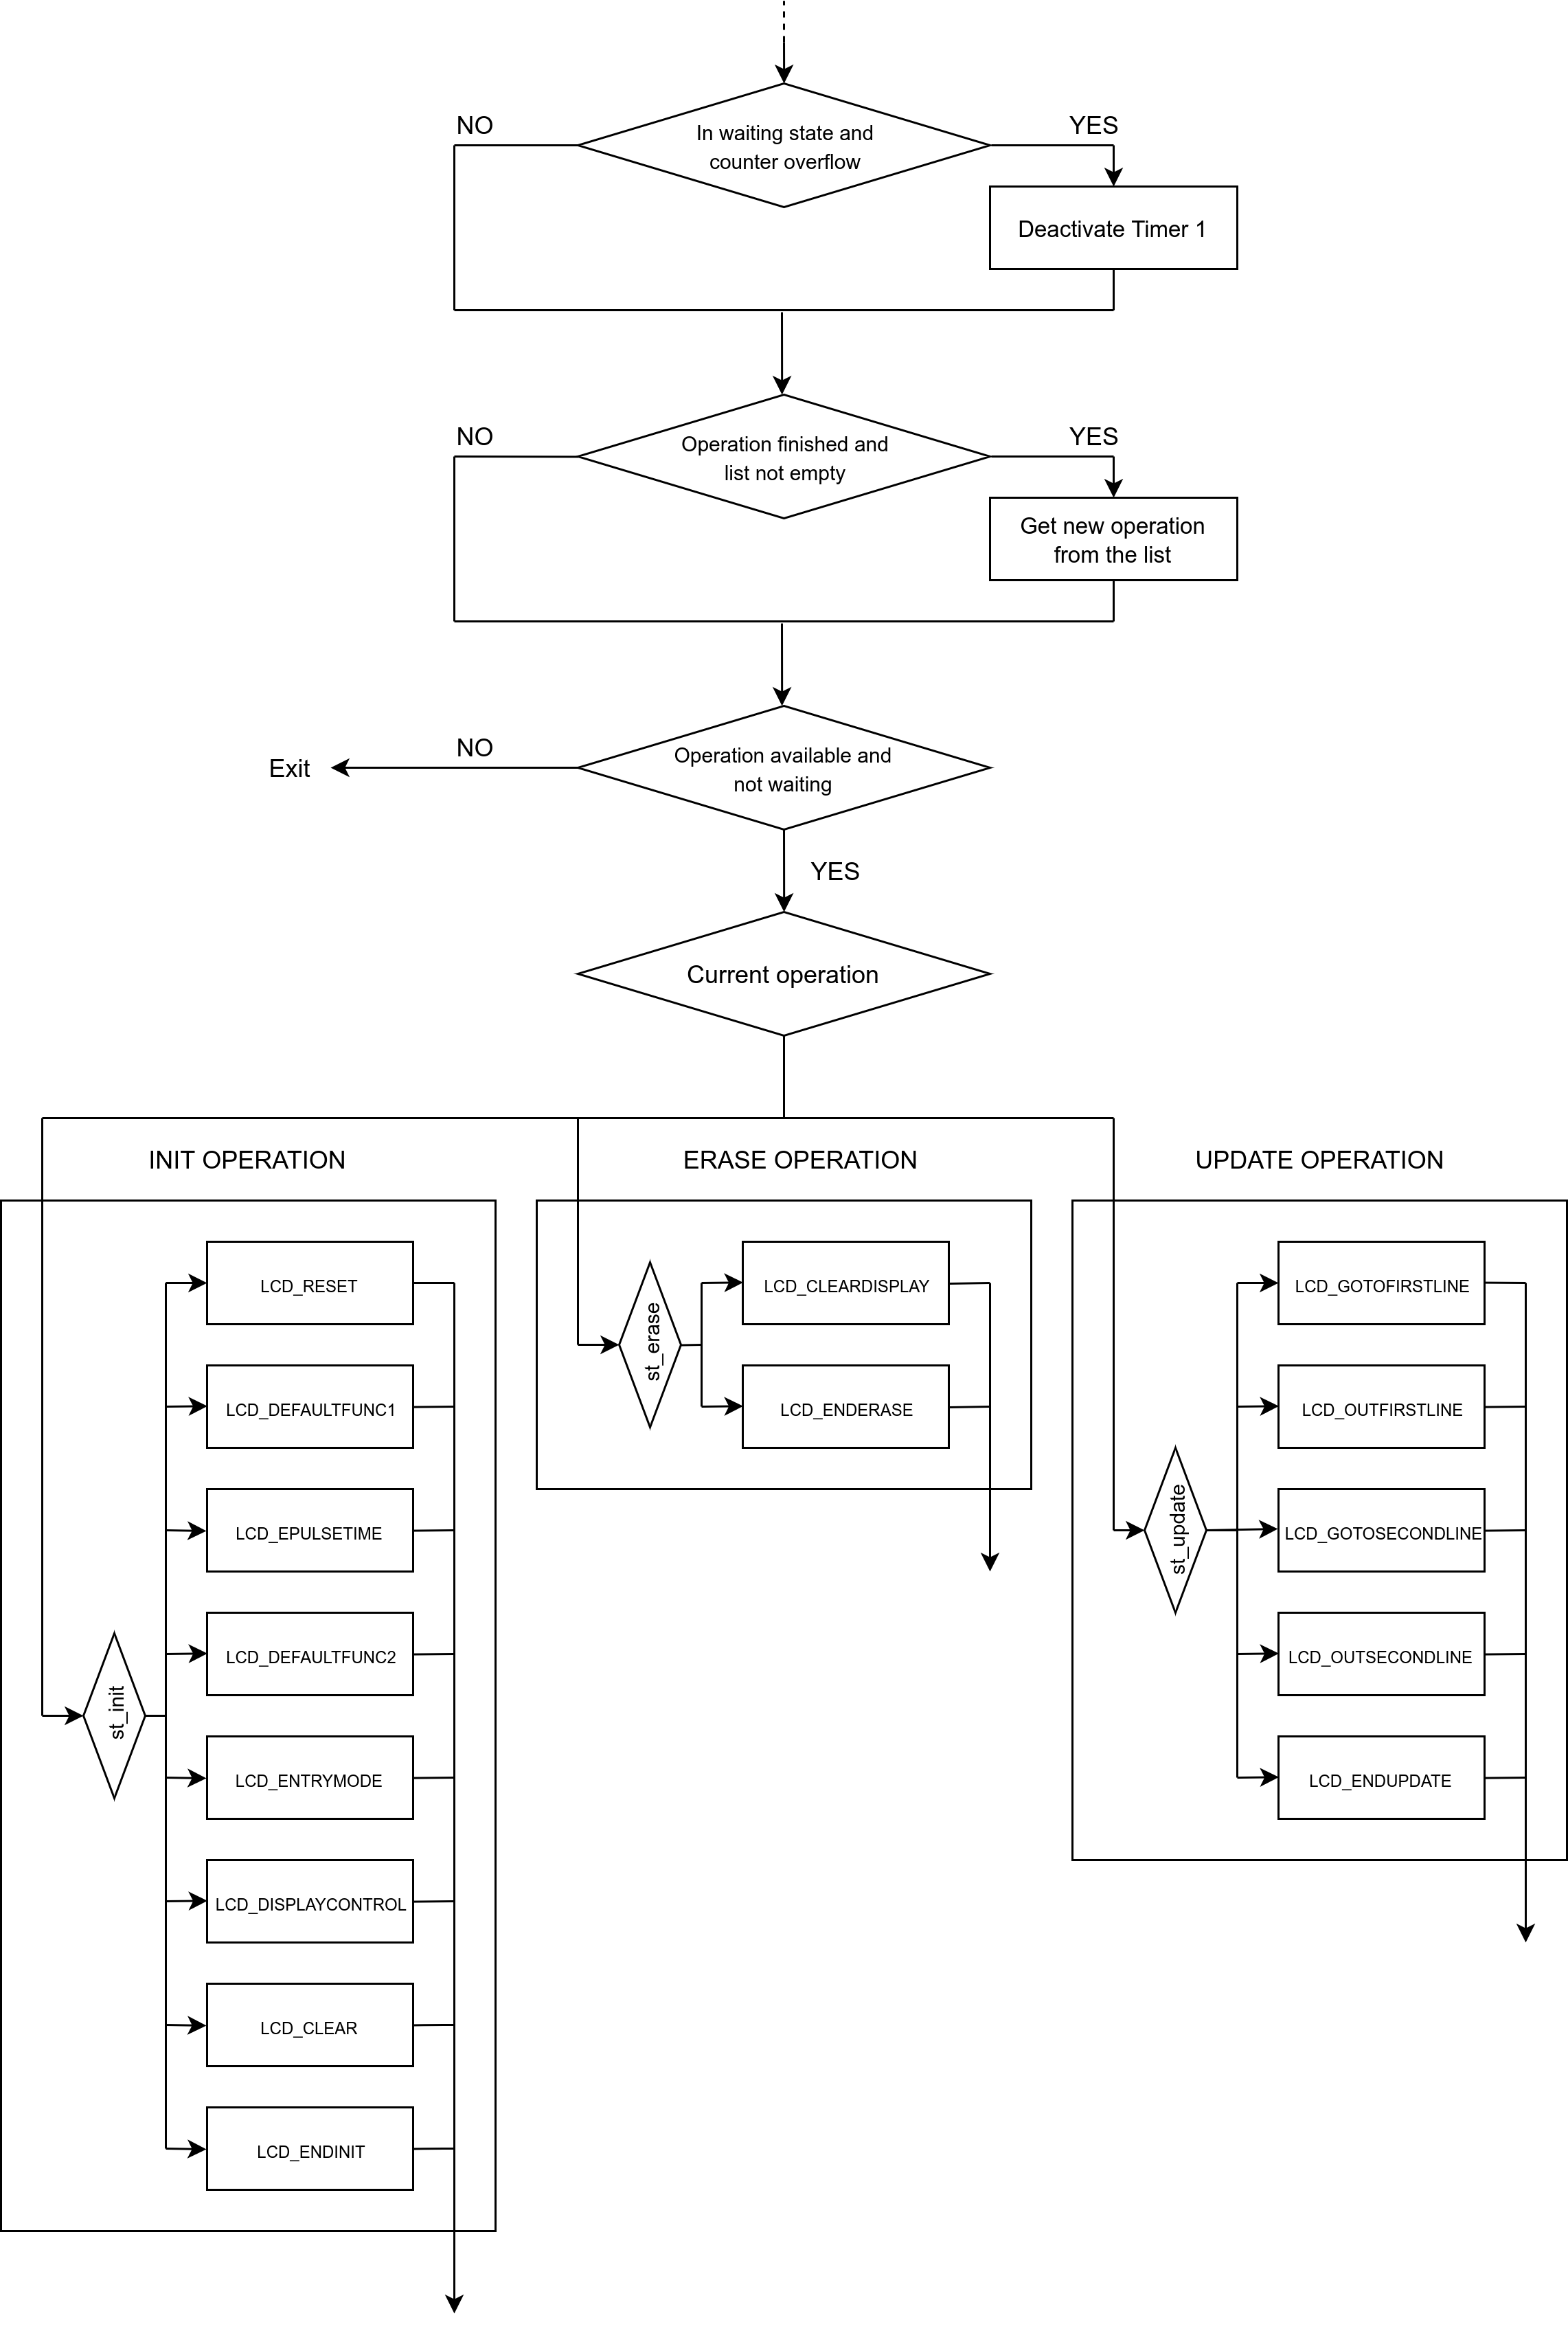
\includegraphics[width=\linewidth]{images/lcdnonblocking2}
	\caption{LCD task instruction flow chart}
	\label{fig:lcdnonblocking2}
\end{figure}

\newpage